% Vehicle Tracking System - Technical Documentation
% LaTeX Template for Academic/Technical Documentation

\documentclass[12pt,a4paper,twoside]{report}

% Required packages
\usepackage[utf8]{inputenc}
\usepackage[T1]{fontenc}
\usepackage{geometry}
\usepackage{fancyhdr}
\usepackage{graphicx}
\usepackage{amsmath,amsfonts,amssymb}
\usepackage{listings}
\usepackage{color}
\usepackage{xcolor}
\usepackage{hyperref}
\usepackage{booktabs}
\usepackage{array}
\usepackage{longtable}
\usepackage{float}
\usepackage{caption}
\usepackage{subcaption}
\usepackage{enumitem}
\usepackage{tikz}
\usepackage{pgfplots}
\usepackage{algorithm}
\usepackage{algorithmic}
\usepackage{minted}
\usepackage{tcolorbox}
\usepackage{natbib}

% Page setup
\geometry{
    left=3cm,
    right=2.5cm,
    top=2.5cm,
    bottom=2.5cm
}

% Header and footer
\pagestyle{fancy}
\fancyhf{}
\fancyhead[LE,RO]{\thepage}
\fancyhead[LO]{\rightmark}
\fancyhead[RE]{\leftmark}
\renewcommand{\headrulewidth}{0.4pt}
\renewcommand{\footrulewidth}{0pt}

% Color definitions
\definecolor{codegreen}{rgb}{0,0.6,0}
\definecolor{codegray}{rgb}{0.5,0.5,0.5}
\definecolor{codepurple}{rgb}{0.58,0,0.82}
\definecolor{backcolour}{rgb}{0.95,0.95,0.92}
\definecolor{primarycolor}{RGB}{0,102,204}
\definecolor{secondarycolor}{RGB}{102,102,102}

% Code listing style
\lstdefinestyle{mystyle}{
    backgroundcolor=\color{backcolour},   
    commentstyle=\color{codegreen},
    keywordstyle=\color{magenta},
    numberstyle=\tiny\color{codegray},
    stringstyle=\color{codepurple},
    basicstyle=\ttfamily\footnotesize,
    breakatwhitespace=false,         
    breaklines=true,                 
    captionpos=b,                    
    keepspaces=true,                 
    numbers=left,                    
    numbersep=5pt,                  
    showspaces=false,                
    showstringspaces=false,
    showtabs=false,                  
    tabsize=2
}
\lstset{style=mystyle}

% Hyperref setup
\hypersetup{
    colorlinks=true,
    linkcolor=primarycolor,
    filecolor=magenta,      
    urlcolor=cyan,
    citecolor=primarycolor,
    pdftitle={Vehicle Tracking System - Technical Documentation},
    pdfauthor={Kasinadh Sarma},
    pdfsubject={Flutter, Firebase, Vehicle Tracking},
    pdfkeywords={Flutter, Firebase, GPS, Vehicle Tracking, Mobile Development}
}

% Custom commands
\newcommand{\code}[1]{\texttt{#1}}
\newcommand{\file}[1]{\texttt{\textbf{#1}}}
\newcommand{\package}[1]{\texttt{\textit{#1}}}
\newcommand{\flutter}{\textsc{Flutter}}
\newcommand{\firebase}{\textsc{Firebase}}
\newcommand{\dart}{\textsc{Dart}}

% Title page information
\title{
    \Huge \textbf{Vehicle Tracking System} \\
    \Large Real-time GPS Fleet Management Solution \\
    \vspace{0.5cm}
    \large Technical Documentation
}
\author{
    \textbf{Kasinadh Sarma} \\
    \small Software Developer \\
    \small \href{mailto:your.email@example.com}{your.email@example.com}
}
\date{\today}

% Custom title page
\makeatletter
\def\maketitle{%
    \null
    \thispagestyle{empty}%
    \vfill
    \begin{center}\leavevmode
        \normalfont
        {\LARGE \@title\par}%
        \hrulefill\par
        {\large \@author\par}%
        \vskip 1cm%
        {\large \@date\par}%
    \end{center}%
    \vfill
    \null
    \cleardoublepage
}
\makeatother

\begin{document}

% Title page
\maketitle

% Abstract
\begin{abstract}
This document presents a comprehensive technical analysis of the Vehicle Tracking System, a real-time GPS fleet management solution developed using the \flutter{} framework and \firebase{} backend services. The system provides cross-platform mobile applications, web dashboards, and desktop applications for comprehensive vehicle fleet monitoring and management.

The implementation leverages modern cloud-native architecture principles, incorporating serverless computing, real-time databases, and advanced geospatial processing capabilities. Key features include real-time GPS tracking with 30-second update intervals, interactive mapping interfaces, driver behavior analysis, geofencing capabilities, and comprehensive reporting systems.

This documentation covers the complete development lifecycle, from initial requirements analysis and system architecture design to implementation details, testing strategies, and performance optimization techniques. The project demonstrates the practical application of cutting-edge mobile development technologies in creating enterprise-grade fleet management solutions.

\textbf{Keywords:} Flutter, Firebase, Vehicle Tracking, GPS, Mobile Development, Real-time Systems, Fleet Management, Cross-platform Development
\end{abstract}

% Table of Contents
\tableofcontents
\listoffigures
\listoftables
\lstlistoflistings

% Main content chapters
% Chapters
\chapter{Introduction}
\label{ch:introduction}

\section{Project Overview}
\label{sec:project_overview}

The Vehicle Tracking System represents a comprehensive, real-time GPS fleet management solution engineered using the \flutter{} framework and \firebase{} backend services. This system delivers live vehicle monitoring, driver behavior analysis, route optimization, and advanced reporting capabilities across multiple platforms including mobile, web, and desktop applications.

\begin{figure}[H]
    \centering
    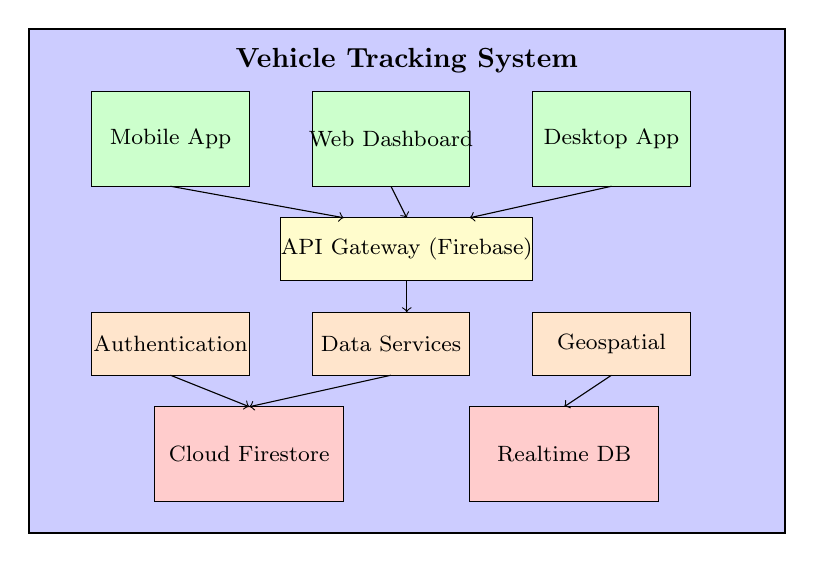
\begin{tikzpicture}[scale=0.8]
        % System overview diagram
        \draw[thick, fill=blue!20] (0,0) rectangle (12,8);
        \node at (6,7.5) {\textbf{Vehicle Tracking System}};
        
        % Client layer
        \draw[fill=green!20] (1,5.5) rectangle (3.5,7);
        \node at (2.25,6.25) {\footnotesize Mobile App};
        
        \draw[fill=green!20] (4.5,5.5) rectangle (7,7);
        \node at (5.75,6.25) {\footnotesize Web Dashboard};
        
        \draw[fill=green!20] (8,5.5) rectangle (10.5,7);
        \node at (9.25,6.25) {\footnotesize Desktop App};
        
        % API Gateway
        \draw[fill=yellow!20] (4,4) rectangle (8,5);
        \node at (6,4.5) {\footnotesize API Gateway (Firebase)};
        
        % Backend services
        \draw[fill=orange!20] (1,2.5) rectangle (3.5,3.5);
        \node at (2.25,3) {\footnotesize Authentication};
        
        \draw[fill=orange!20] (4.5,2.5) rectangle (7,3.5);
        \node at (5.75,3) {\footnotesize Data Services};
        
        \draw[fill=orange!20] (8,2.5) rectangle (10.5,3.5);
        \node at (9.25,3) {\footnotesize Geospatial};
        
        % Database layer
        \draw[fill=red!20] (2,0.5) rectangle (5,2);
        \node at (3.5,1.25) {\footnotesize Cloud Firestore};
        
        \draw[fill=red!20] (7,0.5) rectangle (10,2);
        \node at (8.5,1.25) {\footnotesize Realtime DB};
        
        % Arrows
        \draw[->] (2.25,5.5) -- (5,5);
        \draw[->] (5.75,5.5) -- (6,5);
        \draw[->] (9.25,5.5) -- (7,5);
        \draw[->] (6,4) -- (6,3.5);
        \draw[->] (2.25,2.5) -- (3.5,2);
        \draw[->] (5.75,2.5) -- (3.5,2);
        \draw[->] (9.25,2.5) -- (8.5,2);
    \end{tikzpicture}
    \caption{Vehicle Tracking System High-Level Architecture}
    \label{fig:system_overview}
\end{figure}

\section{Project Background}
\label{sec:project_background}

The transportation and logistics industry has experienced unprecedented growth, driven by e-commerce expansion and globalization. Traditional vehicle tracking methods have proven inadequate for modern business requirements, necessitating intelligent, real-time solutions that can adapt to dynamic operational needs.

\subsection{Market Context}
The global vehicle tracking system market, valued at USD 2.94 billion in 2022, is projected to reach USD 6.04 billion by 2030, exhibiting a CAGR of 9.4\% during the forecast period \cite{market_research_2023}. This growth is attributed to:

\begin{itemize}
    \item Increasing demand for fleet optimization and fuel cost reduction
    \item Growing emphasis on driver safety and behavior monitoring
    \item Rising adoption of IoT and cloud-based solutions
    \item Regulatory requirements for commercial vehicle monitoring
\end{itemize}

\subsection{Technology Evolution}
The evolution of mobile technologies has created unprecedented opportunities for developing sophisticated tracking solutions:

\begin{table}[H]
    \centering
    \caption{Technology Evolution in Vehicle Tracking}
    \label{tab:tech_evolution}
    \begin{tabular}{@{}llll@{}}
        \toprule
        \textbf{Generation} & \textbf{Technology} & \textbf{Capabilities} & \textbf{Limitations} \\
        \midrule
        1st Gen & GPS + GSM & Basic location tracking & High latency, limited features \\
        2nd Gen & GPS + 3G & Real-time updates & Expensive, complex integration \\
        3rd Gen & Smartphone-based & Multi-platform apps & Battery dependency \\
        4th Gen & Cloud-native & Real-time analytics & Requires internet connectivity \\
        \bottomrule
    \end{tabular}
\end{table}

\section{Problem Domain}
\label{sec:problem_domain}

The transportation and logistics industry confronts several critical challenges that traditional tracking systems fail to address adequately:

\subsection{Operational Inefficiencies}
\begin{enumerate}
    \item \textbf{Limited Real-time Visibility}: Traditional systems provide updates with significant delays (5-15 minutes), hindering real-time decision making.
    \item \textbf{Fragmented Data Systems}: Multiple disconnected platforms create operational silos and increase administrative overhead.
    \item \textbf{Poor Route Optimization}: Manual route planning leads to increased fuel consumption and delivery delays.
\end{enumerate}

\subsection{Technical Limitations}
\begin{enumerate}
    \item \textbf{Scalability Constraints}: Legacy systems struggle with growing fleet sizes and increasing data volumes.
    \item \textbf{Integration Challenges}: Limited API access and poor documentation complicate system integration.
    \item \textbf{Mobile User Experience}: Most solutions prioritize web interfaces over mobile optimization.
\end{enumerate}

\section{Solution Approach}
\label{sec:solution_approach}

Our Vehicle Tracking System addresses these challenges through a comprehensive approach leveraging modern technologies:

\subsection{Core Innovations}
\begin{description}
    \item[Real-time Architecture] Utilizing \firebase{} Realtime Database for sub-30-second location updates
    \item[Cross-platform Consistency] Single \flutter{} codebase ensuring identical functionality across platforms
    \item[Cloud-native Design] Serverless architecture enabling automatic scaling and cost optimization
    \item[Mobile-first Approach] Optimized user experience for mobile users with web as secondary interface
\end{description}

\subsection{Technical Advantages}
The system incorporates several technical innovations:

\begin{lstlisting}[language=Dart, caption={Real-time Location Update Implementation}, label={lst:realtime_update}]
class LocationService {
  static const Duration _updateInterval = Duration(seconds: 30);
  
  Stream<Position> getLocationStream() {
    return Geolocator.getPositionStream(
      locationSettings: LocationSettings(
        accuracy: LocationAccuracy.high,
        distanceFilter: 10, // meters
        timeLimit: _updateInterval,
      ),
    );
  }
  
  Future<void> updateRealtimeLocation(
    String vehicleId, 
    LocationModel location
  ) async {
    await FirebaseDatabase.instance
        .ref('live_tracking/$vehicleId')
        .set({
      'latitude': location.latitude,
      'longitude': location.longitude,
      'timestamp': ServerValue.timestamp,
      'speed': location.speed,
      'heading': location.heading,
    });
  }
}
\end{lstlisting}

\section{Key Stakeholders}
\label{sec:stakeholders}

The system serves multiple stakeholder groups with distinct requirements:

\subsection{Primary Users}
\begin{description}
    \item[Fleet Managers] System administrators responsible for overall fleet operations and strategic decision-making
    \item[Drivers] Mobile app users providing location data and receiving navigation assistance
    \item[Dispatchers] Personnel responsible for real-time monitoring and route optimization
    \item[Business Owners] Executive dashboard users requiring high-level analytics and ROI metrics
\end{description}

\subsection{Secondary Users}
\begin{description}
    \item[Maintenance Teams] Personnel responsible for vehicle health monitoring and maintenance scheduling
    \item[Customers] End recipients requiring delivery tracking and estimated time of arrival (ETA) information
    \item[Regulatory Bodies] Organizations requiring compliance reporting and audit capabilities
\end{description}

\section{Document Organization}
\label{sec:document_organization}

This technical documentation is structured to provide comprehensive coverage of the Vehicle Tracking System development:

\begin{description}
    \item[Chapter \ref{ch:literature_review}] Examines existing solutions and identifies research gaps
    \item[Chapter \ref{ch:problem_statement}] Details problem definition and requirements analysis
    \item[Chapter \ref{ch:objectives}] Establishes project goals and success criteria
    \item[Chapter \ref{ch:methodology}] Outlines development methodologies and processes
    \item[Chapter \ref{ch:system_architecture}] Presents technical architecture and design decisions
    \item[Chapter \ref{ch:implementation}] Details implementation specifics and code examples
    \item[Chapter \ref{ch:testing}] Describes testing strategies and quality assurance
    \item[Chapter \ref{ch:results}] Analyzes performance metrics and system evaluation
    \item[Chapter \ref{ch:future_scope}] Discusses enhancement opportunities and roadmap
\end{description}

The documentation follows IEEE standards for technical documentation and incorporates academic research methodologies to ensure comprehensive coverage and reproducibility of results.

\input{chapters/02_literature_review}
\input{chapters/03_problem_statement}
\input{chapters/04_objectives}
\input{chapters/05_methodology}
\input{chapters/06_system_architecture_design}
\input{chapters/07_implementation}
\input{chapters/08_testing_validation}
\input{chapters/09_results_analysis}
\input{chapters/10_future_scope}
\input{chapters/11_source_code_structure}
\input{chapters/12_installation_setup}
\input{chapters/13_performance_benchmarks}
\input{chapters/02_literature_review}
\input{chapters/03_problem_statement}
\input{chapters/04_objectives}
\input{chapters/05_methodology}
\input{chapters/06_system_architecture}
\input{chapters/07_implementation}
\input{chapters/08_testing_validation}
\input{chapters/09_results_analysis}
\input{chapters/10_future_scope}
\input{chapters/11_source_code_structure}
\input{chapters/12_installation_setup}
\input{chapters/13_performance_benchmarks}

% Appendices
\appendix
\input{appendices/a_api_documentation}
\input{appendices/b_database_schema}
\input{appendices/c_configuration_files}
\input{appendices/d_deployment_scripts}

% Bibliography
\bibliographystyle{ieeetr}
\bibliography{references}

\end{document}
